\documentclass[12pt]{article}
%%%%%%%%%%%%%%%%%%%%%%%%%%%%%%%%%%%%%%%%%%%%%%%%%%%%%%%%%%%%%
% Meta informations:
\newcommand{\trauthor}{Michael Hüppe}
\newcommand{\trtype}{Paper} %{Expos\'{e}} %{Review}
\newcommand{\trtitle}{Diffusion Model for Generating new Pokémon}
\newcommand{\trdate}{08.12.2023}

%%%%%%%%%%%%%%%%%%%%%%%%%%%%%%%%%%%%%%%%%%%%%%%%%%%%%%%%%%%%%
% Languages:

% Falls die Ausarbeitung in Deutsch erfolgt:
% \usepackage[german]{babel}
% \usepackage[T1]{fontenc}
% \usepackage[latin1]{inputenc}
% \usepackage[latin9]{inputenc}	 				
% \selectlanguage{german}

% If the thesis is written in English:
\usepackage[english]{babel} 
\usepackage{acronym}

% Define abbreviations using \acrodef{<label>}{<abbreviation>}
\acrodef{HTML}{Hypertext Markup Language}
\acrodef{GAN}{Generative Adversarial Network}
\acrodef{DCGAN}{Deep Convolutional Generative Adversarial Network}
\acrodef{DDPM}{Denoising Diffusion Probabilistic Models}
\acrodef{MSE}{Mean-square Error}
\acrodef{CIFAR-10}{Canadian Institute for Advanced Research - 10}
\acrodef{EMA}{Exponential Moving Average}
\usepackage{enumitem}				
\selectlanguage{english}

%%%%%%%%%%%%%%%%%%%%%%%%%%%%%%%%%%%%%%%%%%%%%%%%%%%%%%%%%%%%%
% Bind packages:
\usepackage{acronym}                    % Acronyms
\usepackage{algorithmic}								% Algorithms and Pseudocode
\usepackage{algorithm}									% Algorithms and Pseudocode
\usepackage{amsfonts}                   % AMS Math Packet (Fonts)
\usepackage{amsmath}                    % AMS Math Packet
\usepackage{amssymb}                    % Additional mathtical symbols
\usepackage{hyperref}             % Additional mathematical symbols
\usepackage{amsthm}
\usepackage{booktabs}                   % Nicer tables
%\usepackage[font=small,labelfont=bf]{caption} % Numbered captions for figures
\usepackage{color}                      % Enables defining of colors via \definecolor
\definecolor{uhhRed}{RGB}{254,0,0}		  % Official Uni Hamburg Red
\definecolor{uhhGrey}{RGB}{122,122,120} % Official Uni Hamburg Grey
\usepackage{fancybox}                   % Gleichungen einrahmen
\usepackage{fancyhdr}										% Packet for nicer headers
%\usepackage{fancyheadings}             % Nicer numbering of headlines

%\usepackage[outer=3.35cm]{geometry} 	  % Type area (size, margins...) !!!Release version
%\usepackage[outer=2.5cm]{geometry} 		% Type area (size, margins...) !!!Print version
%\usepackage{geometry} 									% Type area (size, margins...) !!!Proofread version
\usepackage[outer=3.15cm]{geometry} 	  % Type area (size, margins...) !!!Draft version
\geometry{a4paper,body={5.8in,9in}}

\usepackage{graphicx}                   % Inclusion of graphics
%\usepackage{latexsym}                  % Special symbols
\usepackage{longtable}									% Allow tables over several parges
\usepackage{listings}                   % Nicer source code listings
\usepackage{multicol}										% Content of a table over several columns
\usepackage{multirow}										% Content of a table over several rows
\usepackage{rotating}										% Alows to rotate text and objects
\usepackage[hang]{subfigure}            % Allows to use multiple (partial) figures in a fig
%\usepackage[font=footnotesize,labelfont=rm]{subfig}	% Pictures in a floating environment
\usepackage{tabularx}										% Tables with fixed width but variable rows
\usepackage{url,xspace,boxedminipage}   % Accurate display of URLs

%%%%%%%%%%%%%%%%%%%%%%%%%%%%%%%%%%%%%%%%%%%%%%%%%%%%%%%%%%%%%
% Configurationen:

\hyphenation{whe-ther} 									% Manually use: "\-" in a word: Staats\-ver\-trag

%\lstloadlanguages{C}                   % Set the default language for listings
\DeclareGraphicsExtensions{.pdf,.svg,.jpg,.png,.eps} % first try pdf, then eps, png and jpg
\graphicspath{{./src/}} 								% Path to a folder where all pictures are located
\pagestyle{fancy} 											% Use nicer header and footer

% Redefine the environments for floating objects:
\setcounter{topnumber}{3}
\setcounter{bottomnumber}{2}
\setcounter{totalnumber}{4}
\renewcommand{\topfraction}{0.9} 			  %Standard: 0.7
\renewcommand{\bottomfraction}{0.5}		  %Standard: 0.3
\renewcommand{\textfraction}{0.1}		  	%Standard: 0.2
\renewcommand{\floatpagefraction}{0.8} 	%Standard: 0.5

% Tables with a nicer padding:
\renewcommand{\arraystretch}{1.2}

%%%%%%%%%%%%%%%%%%%%%%%%%%%%
% Additional 'theorem' and 'definition' blocks:
\theoremstyle{plain}
\newtheorem{theorem}{Theorem}[section]
%\newtheorem{theorem}{Satz}[section]		% Inn in Deutsch geschrieben wird.
\newtheorem{axiom}{Axiom}[section] 	
%\newtheorem{axiom}{Fakt}[chapter]			% Inn in Deutsch geschrieben wird.
%Usage:%\begin{axiom}[optional description]%Main part%\end{fakt}

\theoremstyle{definition}
\newtheorem{definition}{Definition}[section]

%Additional types of axioms:
\newtheorem{lemma}[axiom]{Lemma}
\newtheorem{observation}[axiom]{Observation}

%Additional types of definitions:
\theoremstyle{remark}
%\newtheorem{remark}[definition]{Bemerkung} % Inn in Deutsch geschrieben wird.
\newtheorem{remark}[definition]{Remark} 

%%%%%%%%%%%%%%%%%%%%%%%%%%%%
% Provides TODOs within the margin:
\newcommand{\TODO}[1]{\marginpar{\emph{\small{{\bf TODO: } #1}}}}

%%%%%%%%%%%%%%%%%%%%%%%%%%%%
% Abbreviations and mathematical symbols
\newcommand{\modd}{\text{ mod }}
\newcommand{\RS}{\mathbb{R}}
\newcommand{\NS}{\mathbb{N}}
\newcommand{\ZS}{\mathbb{Z}}
\newcommand{\dnormal}{\mathit{N}}
\newcommand{\duniform}{\mathit{U}}

\newcommand{\erdos}{Erd\H{o}s}
\newcommand{\renyi}{-R\'{e}nyi}
\usepackage[backend=biber,style=apa, natbib=true]{biblatex}
\DefineBibliographyStrings{english}{andothers = {\emph{et al}\adddot}}
\addbibresource{main.bib} % The filename of the bibliography
%%%%%%%%%%%%%%%%%%%%%%%%%%%%%%%%%%%%%%%%%%%%%%%%%%%%%%%%%%%%%
% Document:
\begin{document}
\renewcommand{\headheight}{14.5pt}

\fancyhead{}
\fancyhead[CO]{\trtitle}

%%%%%%%%%%%%%%%%%%%%%%%%%%%%
% Cover Header:
\title{\trtitle\\[0.3cm]{\normalsize\trtype}}
\author{\trauthor}
\date{\trdate}
\maketitle

%%%%%%%%%%%%%%%%%%%%%%%%%%%%

\thispagestyle{empty}
\pagenumbering{arabic}
%
%% Abstrt gives a brief summary of the main points of a paper:
\begin{abstract}
Making its gaming debut in 1996 with "Pokémon Red and Green" and earning approximately 368 million from game sales alone, the Pokémon series stands as one of Nintendo's oldest and most well-known franchises. With a unique blend of character designs and turn-based role-playing, the game introduced an entire generation to a distinctive gaming style, earning its place as the seventh most successful game of all time. Consequently, the franchise's current cultural significance comes as no surprise.

The community's embrace of "Fakémons," or self-made Pokémon, has reached a point where these creations feature prominently in entire fan-made games. This widespread enthusiasm paved the way for the exploration of generating new Pokémon through the application of deep learning. In recent years the generation of images has become more popular with the easy access to generative networks such as \href{https://openai.com/blog/dall-e/}{DALL-E}, \href{https://github.com/NVlabs/stylegan2}{StyleGAN2} or \href{https://www.openai.com/research/gpt}{GPT-3}. Diffusion models describe one of the most popular architectures.	This paper outlines the methodology employed for scraping and standardizing the data, along with the construction of the network architecture.\\

\end{abstract}

% the actual content, usually separated over a number of sections
% each section is assigned a label, in order to be able to put a
% crossreference to it

\newpage

\section{Introduction}
\label{sec:introduction}

The following presents the possibility and methodology of using \ac{DDPM} to generate novel designs for Pokémons. Firstly, previous approaches and their used models are presented in Section \ref{sec:relwork}. Following, the methodology is described namely the model architecture in Section \ref{sec:model} and the data acquisition and processing Section \ref{sec:dataAca_and_preprocessing}. Finally, the results are presented and discussed in Section \ref{sec:results} and \ref{sec:discussion}. Section \ref{sec:conclusion} presents the shortcomings of this study and what can be improved upon. 
%
%
\section{Related Work}
\label{sec:relwork}
The following section is divided into two. Firstly, related works regarding \ac{GAN}s are discussed with a closer look into the current uses of \ac{DDPM}s. Secondly, previous approaches using \ac{GAN}s to create new images of Pokémon are analyzed. 
There are multitudes of variation of \ac{GAN}s, with notable architectures like \ac{DCGAN} \citep{Radford2016}, StyleGAN \citep{Karras2019}, and BigGAN \citep{Brock2019}. While all of these models have the same underlying purpose, i.e. generating novel images based on an existing data pool, their architecture has been optimized for a specific task. For example the StyleGan architecture is used for combining images, often applying certain features of one image onto another \citep{Karras2019}. In contrast, the BigGan architecture is used to enhance the quality of images often up-scaling low resolution images to a higher resolution \citep{Brock2019}. \\
Given their ability to model intricate patterns and dependencies within data \ac{DDPM}s have been employed in various tasks. For example, image translation \citep{Sasaki2021}, inpainting \citep{Lugmayr2022} or image restoration \citep{Nair2023}. \ac{DDPM}s have also been used beyond image generation, examples are feature extraction \citep{Bandara2024}, anomaly detection \citep{Wyatt2022} and time-series forecasting \citep{Rasul2021}. Given their variability in use-cases \ac{DDPM}s are a good fit for generating new Pokémon designs. \\


Generating Pokémon using deep learning is not a novel idea. \cite{Kleiber2020} used a \ac{GAN} to create new Pokémon based on a dataset of ~800 data samples. The presented results seen in Figure \ref{fig:kleiberresults} can definitely be approved upon.\\
 

 \begin{figure}[h]
	\centering
	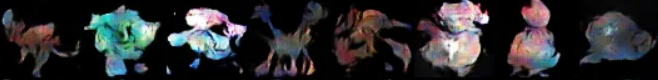
\includegraphics[width=1\linewidth]{src/Images/Kleiber_results}
	\caption[Results of \cite{Kleiber2020}]{Results of \cite{Kleiber2020}. The object somewhat resemble the colour scheme and form of a Pokémons. However, no image is recognizable as a complete design.}
	\label{fig:kleiberresults}
\end{figure}

Using the same dataset \cite{Chambel2022} trained a \ac{DCGAN} and achieved better results. The colour of the generated images is much closer to the often vibrant colour presented in the dataset. The results can be seen in Figure \ref{fig:chambelresults}.

\begin{figure}[h]
	\centering
	
\includegraphics[width=1\linewidth]{src/Images/Chambel_results}
	\caption[Results presented by \cite{Chambel2022}]{Results presented by \cite{Chambel2022}.}
	\label{fig:chambelresults}
\end{figure}


\section{Model}
\label{sec:model}
The model employed was based on the \acf{DDPM} presented by \cite{Ho2020} who presents both an unconditional Model and a conditional one. For generating the images I only employed the conditional architecture. However, the architecture was slightly modified. The most significant change was the implementation of a scale factor which gives the ability to increase/decrease the amount of model parameters.

\ac{DDPM} are a class of generative models that aim to model the data distribution by defining a diffusion process. The primary idea behind \ac{DDPM}s is to transform a simple distribution (e.g., a Gaussian distribution) into the target data distribution through a series of carefully designed transformations. This diffusion process is done step-by-step slowly transforming the input noise to an image resembling the training data. \\
At each step of the diffusion process, a noise is added to the data, and the data is transformed to a new state. This process is repeated multiple times until the input noise has been transformed to an image resembling the training data. \\
The model is trained by optimizing its parameters to maximize the likelihood of the observed data. During training, the model learns the transformations that map the simple initial distribution to the target data distribution. This involves adjusting the parameters in a way that the generated samples match the characteristics of the training data.\\
Once trained, the DDPM can generate new samples by starting with samples from the simple initial distribution and applying the learned reverse transformations in the reverse order.\\
Overall, DDPMs provide a probabilistic framework for generative modeling, leveraging a diffusion process to model the transformation from a simple distribution to a complex data distribution. This allows them to capture intricate patterns and dependencies in the data.\\


The diffusion model approach can be used in combination with a multitude of model architectures. The most common and the model used by us was the U-Net as presented by \cite{Ronneberger2015}. \\
The U-Net is named after the shape of the models' architecture. As a \ac{DDPM} the U-Net aims to predict noise, to achieve this it creates a feature map for the input image. Using convolutions and max-pooling the resolution of the feature map is decreased at each step. This resembles the idea of a decoder to break down each image into it's most important components. Similarly, the U-Net implements an encoding process where resolution of the previously reduced feature map are then increased to replicate an image from decoding noise. This is done by using up-convolutions. Additionally, the U-Net implements skip connections at each resolution change. An original illustration of the U-Net is depicted in Figure \ref{fig:unet}.\\

\begin{figure}[H]
	\centering
	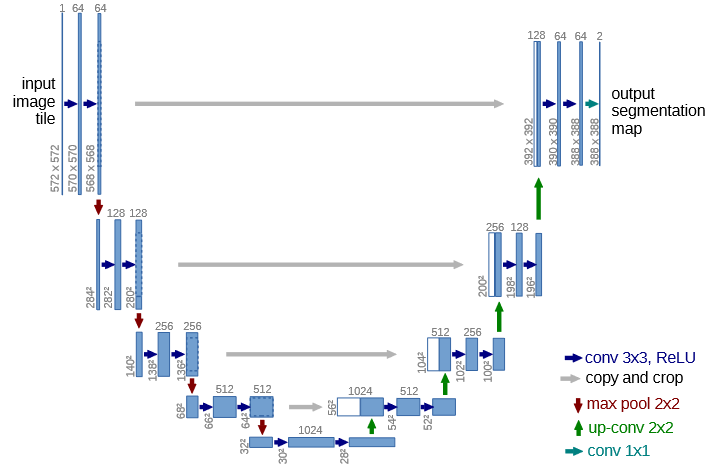
\includegraphics[width=0.7\linewidth]{src/Images/u_net}
	\caption[U-Net architecture]{U-Net architecture as presented by \cite{Ronneberger2015}.}
	\label{fig:unet}
\end{figure}


\section{Data Acquisition and Preprocessing}
\label{sec:dataAca_and_preprocessing}
\subsection{Acquisition}
There is no official Pokémon dataset that provides the extensive sample size typically required for training generative deep learning models \citep{Yang2023}. Most of the available datasets offer only one image per Pokémon, resulting in approximately 1000 images in total. In comparison, the \href{https://www.cs.toronto.edu/~kriz/cifar.html}{\ac{CIFAR-10}} dataset consists of 60,000 samples. Moreover, each Pokémon has a unique and easily distinguishable design, making it challenging to identify similarities between them. To address this limitation, I opted to create my own Pokémon dataset using web scraping.

I used web scraping to extract data from the \href{https://pokemondb.net/}{Pokémon database}, which lists all Pokémon along with various design variations for each. The Python packages \href{https://www.crummy.com/software/BeautifulSoup/bs4/doc/}{BeautifulSoup} and \href{https://requests.readthedocs.io/en/latest/}{requests} packages provide functions to parse the website into \ac{HTML} and identify relevant tags. The \href{https://pokemondb.net/pokedex/national}{national Pokédex} which provides a list of all current Pokémon organized by Generation \footnote{In the context of Pokémon, a "generation" refers to a specific group or series of Pokémon games released by Nintendo and Game Freak. Each generation introduces a new set of Pokémon species, game mechanics, and often a new region to explore.} represents the start point of the acquisition pipeline.

I collected links for each entry, simplifying the retrieval of all accessible images through a systematic naming convention. The link structure is as follows: "pokemondb.net/identifier/Pokémon." Changing the identifier granted access to two distinct datasets. The "artwork" identifier encompassed both official and alternative artwork, while the "sprites" section stored all in-game renditions of the Pokémon. In total, I obtained 26,896 unique images (22,825 sprites and 4,071 artworks). The term "unique" requires caution, as I intentionally included both male and female versions (even if differing by minor details) and normal and shiny versions (same Pokémon but with different color coding). Additionally, the database provides GIFs depicting the idle animation of the Pokémon. The start and middle frame of these animations were added to the dataset. The back view of Pokémon were ignored since the goal was to generate images from the front. 

The code for web scraping the images can be found \href{https://github.com/mhueppe/Diffusion_Models/tree/master/preprocessing}{here}. Figure \ref{fig:variouscharizard} shows an example of artworks and sprites for the Pokémon entry for \href{https://pokemondb.net/pokedex/charizard}{Charizard}.

\begin{figure}[h]
	\centering
	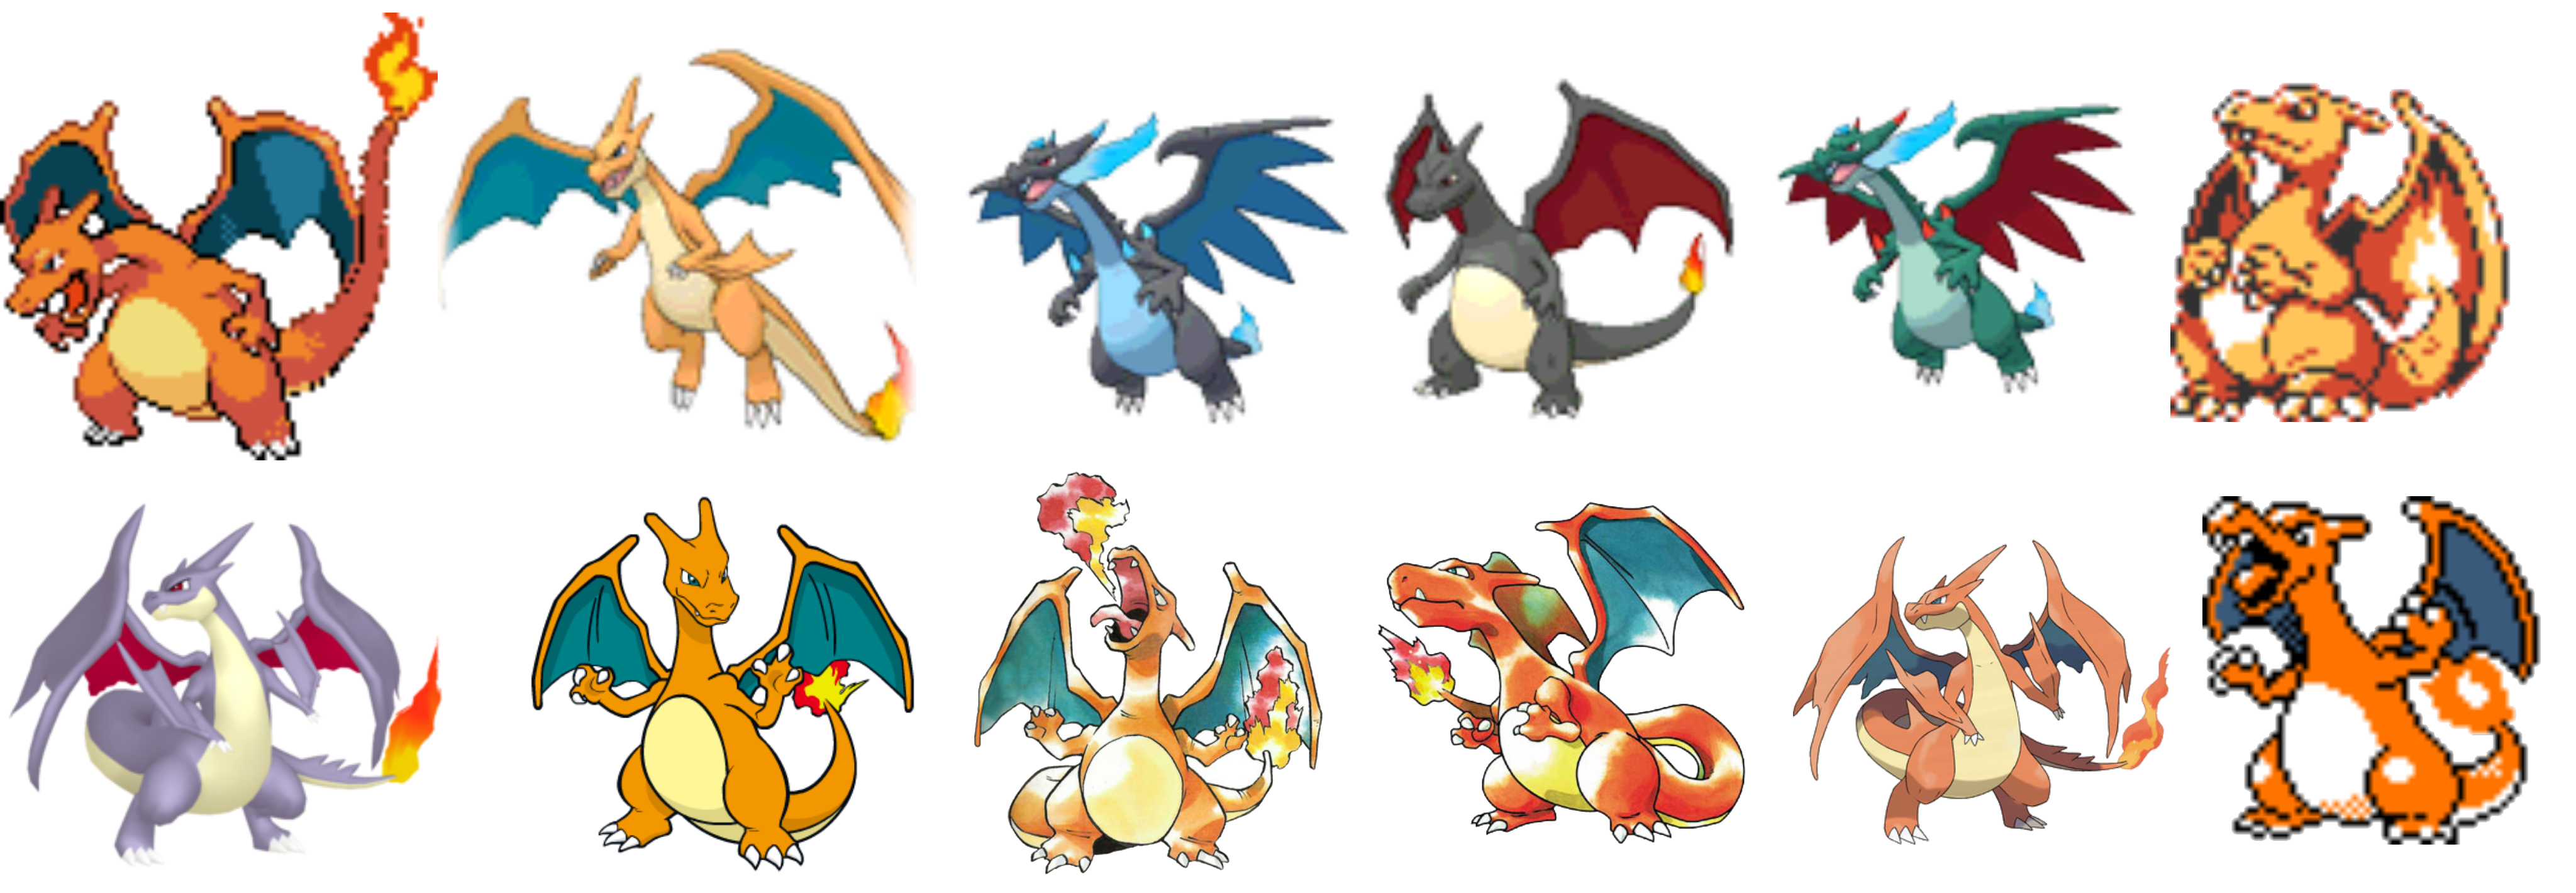
\includegraphics[width=\linewidth]{src/Images/various_charizard}
	\caption[Different Pokémon renditions]{Different renditions of the same Pokémon. Both samples from the artwork and sprite dataset are presented}
	\label{fig:variouscharizard}
\end{figure}

Note that the trained model is a conditional diffusion model, thus the samples should be categorized in a logical scheme.  There are multiple approaches on how the samples can be grouped. Typically, Pokémon are grouped based on their typing \footnote{Typing refers to the elemental or thematic category (fire, water, ghost, fairy etc.) that a Pokémon belongs to. Each Pokémon has one or two types, which determine its strengths and weaknesses in battles. There are 18 different types in total, and each type has its own set of interactions with other types.}. However, optimally similar images are grouped together. Pokémon belonging to the same type can differ drastically in regards to their appearance. Since the goal was to maximize the inner-class visual similarity and the between-class discrepancy, I opted to group samples based on the body from the Pokémon. 
This resulted in following classes.\\

Pokémon with: 

\begin{multicols}{3}
	\begin{enumerate}[itemsep=2pt,parsep=2pt]
		\item \href{https://bulbapedia.bulbagarden.net/wiki/List_of_Pok%C3%A9mon_by_shape#Pok.C3.A9mon_consisting_of_only_a_head}{only a head}
		\item \href{https://bulbapedia.bulbagarden.net/wiki/List_of_Pok%C3%A9mon_by_shape#Pok.C3.A9mon_consisting_of_a_head_and_legs}{a head and legs}
		\item \href{https://bulbapedia.bulbagarden.net/wiki/List_of_Pok%C3%A9mon_by_shape#Pok.C3.A9mon_with_fins}{fins}
		\item \href{https://bulbapedia.bulbagarden.net/wiki/List_of_Pok%C3%A9mon_by_shape#Pok.C3.A9mon_with_an_insectoid_body}{insectoid body}
		\item \href{https://bulbapedia.bulbagarden.net/wiki/List_of_Pok%C3%A9mon_by_shape#Pok.C3.A9mon_with_an_insectoid_body}{quadruped body}
		\item \href{https://bulbapedia.bulbagarden.net/wiki/List_of_Pok%C3%A9mon_by_shape#Pok.C3.A9mon_with_a_single_pair_of_wings}{single pair of wings}
		\item \href{https://bulbapedia.bulbagarden.net/wiki/List_of_Pok%C3%A9mon_by_shape#Pok.C3.A9mon_consisting_of_multiple_bodies}{multiple bodies}
		\item \href{https://bulbapedia.bulbagarden.net/wiki/List_of_Pok%C3%A9mon_by_shape#Pok.C3.A9mon_with_tentacles_or_a_multiped_body}{tentacles}
		\item \href{https://bulbapedia.bulbagarden.net/wiki/List_of_Pok%C3%A9mon_by_shape#Pok.C3.A9mon_consisting_of_a_head_and_a_base}{base and legs}
		\item \href{https://bulbapedia.bulbagarden.net/wiki/List_of_Pok%C3%A9mon_by_shape#Pok.C3.A9mon_with_a_bipedal.2C_tailed_form}{bipedal with tail}
		\item \href{https://bulbapedia.bulbagarden.net/wiki/List_of_Pok%C3%A9mon_by_shape#Pok.C3.A9mon_with_a_bipedal.2C_tailless_form}{ bipedal without tail}
		\item \href{https://bulbapedia.bulbagarden.net/wiki/List_of_Pok%C3%A9mon_by_shape#Pok.C3.A9mon_with_two_or_more_pairs_of_wings}{two or more pairs of wings}
		\item \href{https://bulbapedia.bulbagarden.net/wiki/List_of_Pok%C3%A9mon_by_shape#Pok.C3.A9mon_with_serpentine_bodies}{serpentine body}
		\item \href{https://bulbapedia.bulbagarden.net/wiki/List_of_Pok%C3%A9mon_by_shape#Pok.C3.A9mon_consisting_of_a_head_and_arms}{a head and arms}
	\end{enumerate}
\end{multicols}

\begin{figure}[h]
	\centering
	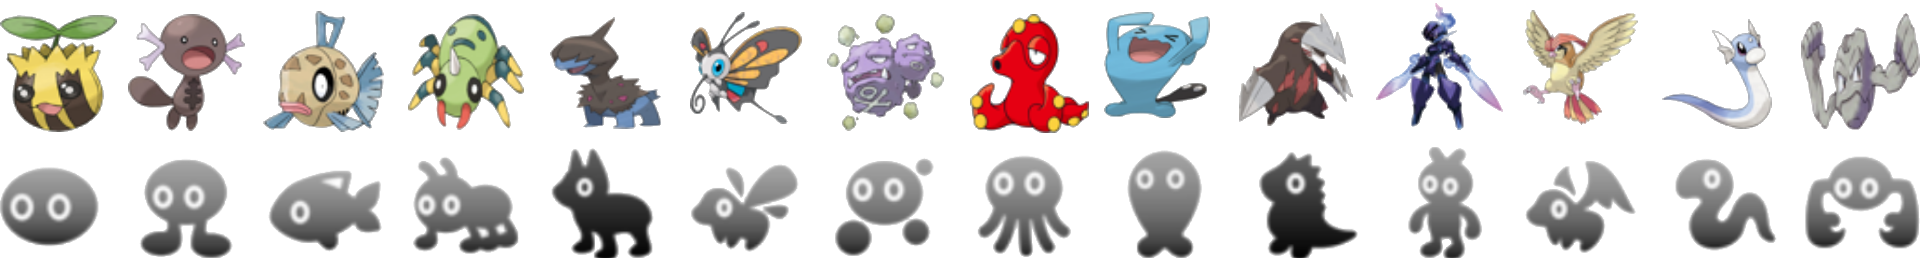
\includegraphics[width=\linewidth]{src/Images/bodyCategorys}
	\caption[Body Categories]{Different body types used to categorise the Pokémon.}
	\label{fig:bodycategorys}
\end{figure}

\subsection{Preprocessing}
The next problem I encountered was the difference in their background, their image mode and
type. At first I resize every image to 64x64. The original artwork and sprites were all transparent ”.png”, meaning they have no background and therefore a fourth channel encoding the transparency of the given pixel. This fourth channel resulted in partially transparent Pokémon and added unnecessary parameters to the network. Therefore I converted each of the ”RGBA”
images to uniform ”RGB” images with a white background to keep their characteristic black outlining. \\
As the alternative artworks were collected from a variety of different artists there was no convention resulting in different file types (jpg, jpeg and vector png), backgrounds and image modes.
To keep the format I established in the previous step I again removed the additional transparency channel and converted each image to png. Additionally, I detected each image which did not have a white background and adjusted it accordingly.\\
 Moreover, was there a difference
in coverage of the image. While the artworks used all available space of the image the sprites only used around 10\% therefore exposing a lot of white background. This was apparent after training a few test epochs which resulted in solely white images with a small focus somewhere in the center (which was no surprise as the sprites represented the majority of the dataset). To counteract this, I located the focus point of the image (location of Pokémon) by removing
each row/column only containing white pixels. Then to avoid morphing the shape of the Pokémon I padded it to a square. At last I again resized the cropped image to get a uniform size of 64x64 pixels.\\
The code for making the images uniform can be found \href{https://github.com/mhueppe/Diffusion_Models/blob/master/preprocessing/preprocessing_uniform_data.py}{here}.

An example for a sample before and after applying the uniform process can be seen in Figure \ref{fig:preprocessingpipeline}.

\begin{figure}[h]
	\centering
	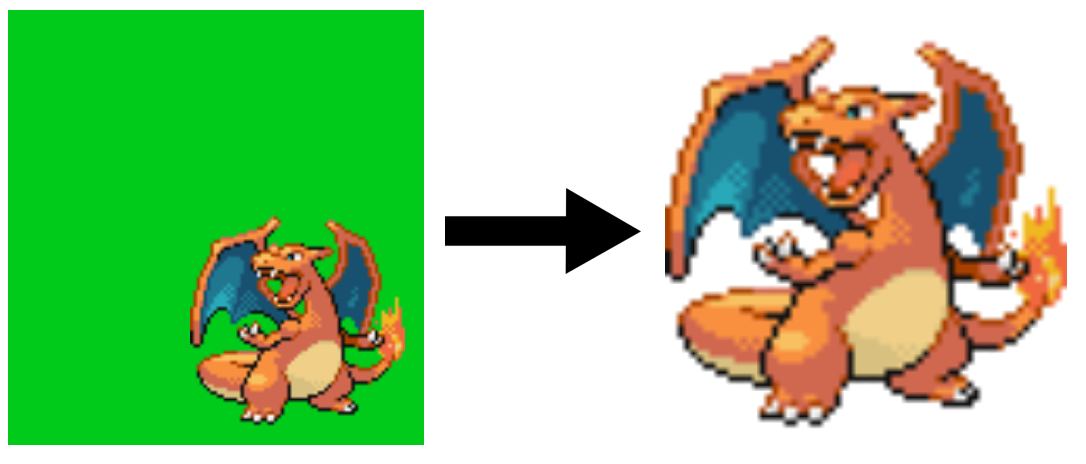
\includegraphics[width=0.5\linewidth]{src/Images/preprocessing_pipeline}
	\caption[Before and After Uniform Process]{A sample before and after applying the uniform process.}
	\label{fig:preprocessingpipeline}
\end{figure}

The previous preprocessing steps  were  done before training the model to ensure that the focus for each samples is on the Pokémon. In addition to this, more preprocessing was done while training to each sample. This included applying a random crop to the image, randomly flipping it on the vertical axis and normalize each colour channel to have a mean of 1 and a standard deviation of 1.


\section{Results}\label{sec:results}
The following describes the results reported on both the \href{https://www.cs.toronto.edu/~kriz/cifar.html}{\ac{CIFAR-10}} dataset and our own Pokémon dataset. Since the quality of the generated image is somewhat subjective the \ac{MSE} during training is presented as well. 


\subsection{\ac{CIFAR-10}}\label{sec:results:cifar10}
To validate the model pipeline I first trained the model on the \href{https://www.cs.toronto.edu/~kriz/cifar.html}{\ac{CIFAR-10}} dataset since the model has already reported good results on this data. The \ac{CIFAR-10} dataset is a collection of 60,000 32x32 color images in 10 different classes, with 6,000 images per class. Each image belongs to one of the following classes:

\begin{multicols}{5}
	\begin{enumerate}[itemsep=2pt,parsep=2pt]
		\item airplane
		\item car
		\item bird
		\item cat
		\item deer
		\item dog
		\item frog 
		\item horse
		\item ship
		\item truck
	\end{enumerate}
\end{multicols}

Similarly, our model reported good results as Ill. 

Figure \ref{fig:cifar10msewithpredictions} shows the change of \ac{MSE} during training. Additionally, epoch 30 and 100 are highlighted with sample images from these epochs. The \ac{MSE} decreases rapidly at the start of the training. For the following epochs the \ac{MSE} hovers around 0.01 and 0.04. While stable within this range there is no steady (in-)decrease. However, the images differ heavily when it comes to resemblance to the training images. 
Figure (TBA) shows the predicted images over time. As one can see the images predicted in the early stages of training  were  not reminiscent of the input data and mostly show either random noise or images containing only one colour. Similar to how the \ac{MSE} decreased over time the quality of the images increased. The final images clearly depict objects of the respected class. 

\begin{figure}[H]
	\centering
	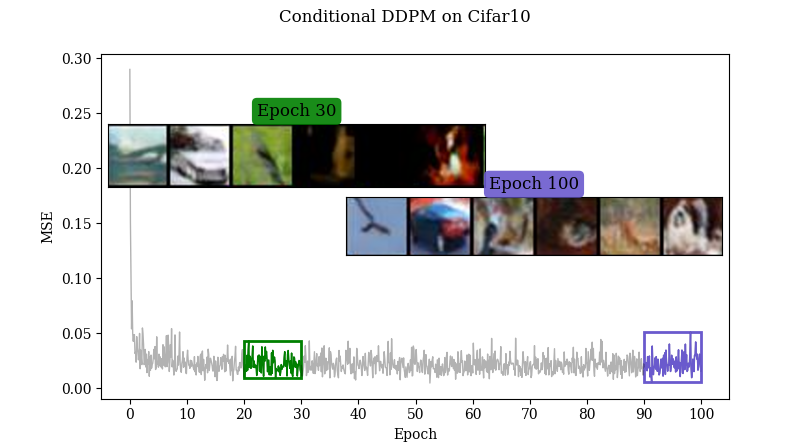
\includegraphics[width=\linewidth]{src/Images/cifar10_mse_with_predictions}
	\caption[\ac{CIFAR-10} \ac{MSE} over time.]{\ac{CIFAR-10} \ac{MSE} over time.}
	\label{fig:cifar10msewithpredictions}
\end{figure}


\begin{figure}[H]
	\centering
	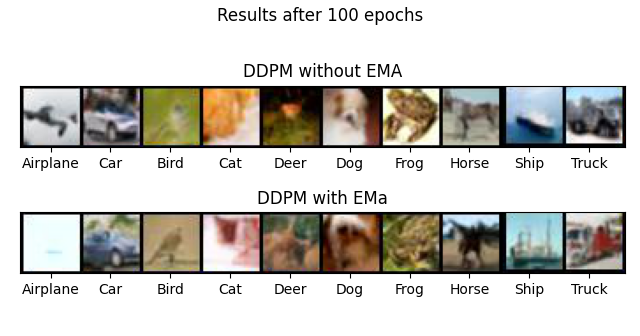
\includegraphics[width=1\linewidth]{src/Images/cifar10_results}
	\caption[Generated \ac{CIFAR-10} images of \ac{DDPM}]{Generated images of \ac{DDPM}}
\label{fig:cifar10results}
\end{figure}

\subsection{Pokémon}\label{sec:pokémon}
The results presented in Section \ref{sec:results:cifar10} validated that the \ac{DDPM} was able to replicate images from the training dataset specific for each class. The following describes model performance on the self-crafted Pokémon dataset. 

Figure \ref{fig:pokemonperbodytype} displays generated images after training for each respective class showing the conditionality of the model. Most generated images resemble the body type they are attributed to. 

\begin{figure}[H]
	\centering
	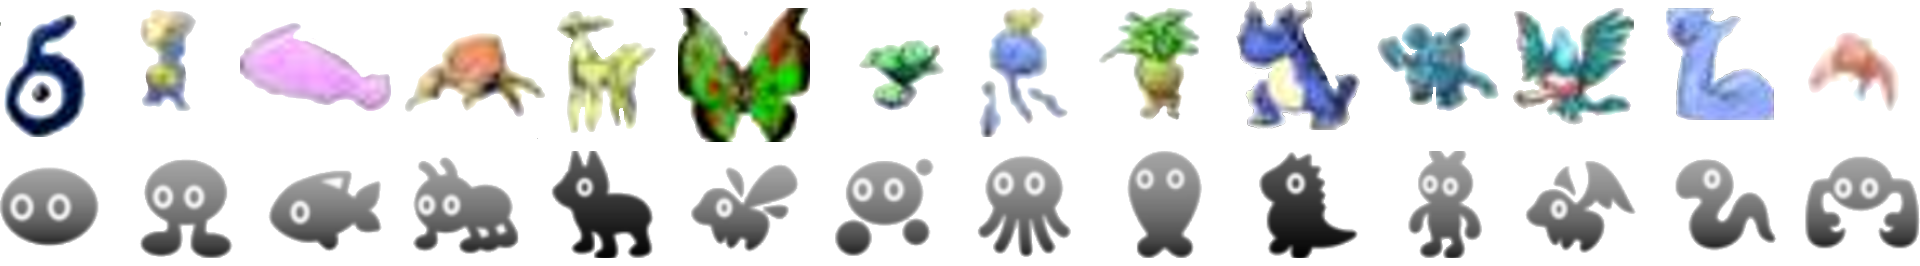
\includegraphics[width=\linewidth]{src/Images/pokemon_per_body_type}
	\caption[Pokémon per body type]{Pokémon per body type.}
	\label{fig:pokemonperbodytype}
\end{figure}

Figure \ref{fig:pokemonmsewithpredictions} shows the change of \ac{MSE} during training. Similarly to Figure \ref{fig:cifar10msewithpredictions} there is a rapid decrease of \ac{MSE} at the start of the training with a \ac{MSE} staying relatively constant. Consistent with the results for the \ac{CIFAR-10} dataset the images keep improving even though the loss seems to be stagnant. However, there is a variety in quality of generated pictures with respect to class. Namely, the body types with wings seem to be replicated the best.

\begin{figure}[H]
	\centering
	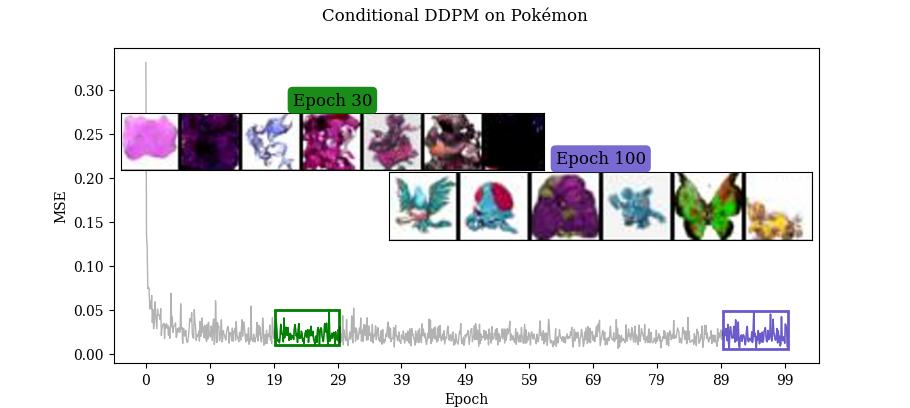
\includegraphics[width=1.1\linewidth]{src/Images/pokemon_mse_with_predictions}
	\caption[Change of \ac{MSE} over time.]{Change of \ac{MSE} over time. The \ac{MSE} values leading up to the 30 and 100 epoch are highlighted. Additionally, generated samples for both highlighted epochs are shown.}
	\label{fig:pokemonmsewithpredictions}
\end{figure}

A known problem with \ac{GAN}s is mode collapse \citep{Zhang2018}. This phenomenon describes models which focus on the most common feature in the dataset to generate new images. Instead of generating diverse samples that cover the entire data distribution, the generator might focus on generating samples with certain features. This lack of diversity in the generated data can be seen in the class "only head".\\
This category includes the Pokémon \href{https://bulbapedia.bulbagarden.net/wiki/Unown_(Pok%C3%A9mon)}{"Unown"}, which mimics the Latin alphabet and thus has 28 variations. Though different, all variations follow the same design rules, black lines and one eye. Accounting for all different image types 53\% of the images in this category were just depicting some variation of this Pokémon. This can be seen in the results generated for this class. Mainly, most of th generated images follow the "Unown" design. Examples can be seen in Figure \ref{fig:Unownvariety}. 

\begin{figure}[H]
	\centering
	
\includegraphics[width=0.8\linewidth]{src/Images/unown_examples}
	\caption[Generated images for head]{Different generated images for the head category reminiscent of the Pokémon "Unown".}
	\label{fig:Unownvariety}
\end{figure}


Moreover, there is a noticeable difference in the coherence of images among classes. Images generated for a specific class exhibit greater similarities, whereas other classes display a higher variance in the generated images. This is illustrated in Figure \ref{fig:categorycomparison}. The samples generated for the class "quadrupled" differ more strongly in comparison to images generated for the class "winged".


\begin{figure}[H]
	\centering
	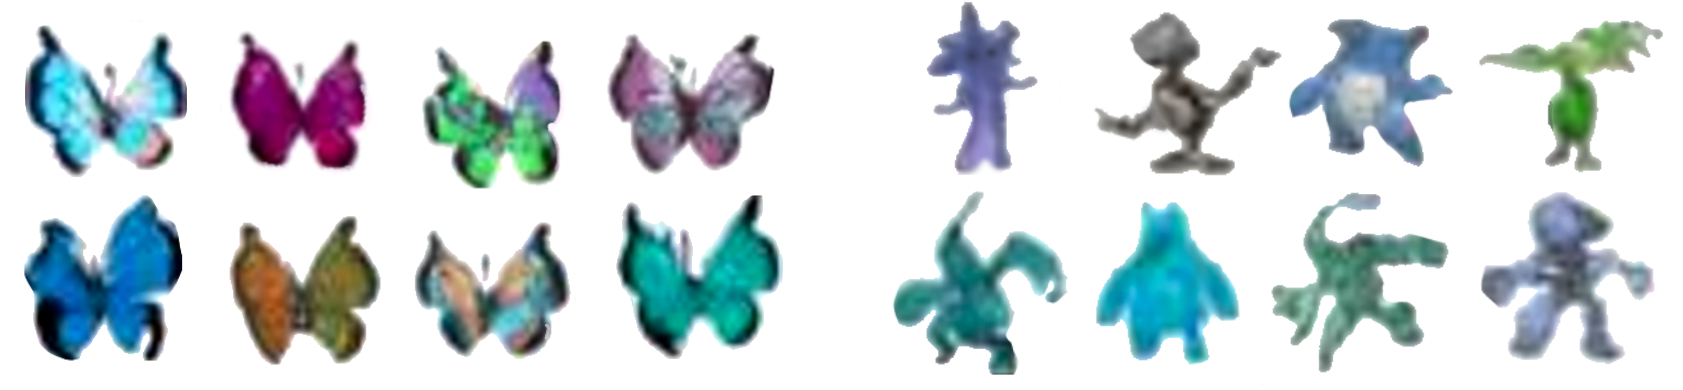
\includegraphics[width=0.9\linewidth]{src/Images/category_comparison}
	\caption[Class Comparison]{Comparison between classes "with wings" (left) and "bipedal without tail" (right).}
	\label{fig:categorycomparison}
\end{figure}

\section{Discussion}
\label{sec:discussion}
Our model demonstrated comparable performance on both the benchmark dataset and our custom created dataset. The incorporation of the diffusion model and the expansion of the dataset proved to exert a positive influence on the quality of the predicted images. Notably, our images exhibited a more refined design compared to previous studies (refer to Figure \ref{fig:kleiberresults} \& \ref{fig:chambelresults}). This outcome was anticipated, as generative models tend to excel when operating with larger datasets \citep{Yang2023}. Furthermore, it is noteworthy that \ac{DDPM}s exhibited the capability to generate images of higher quality compared to simpler \ac{GAN}s \citep{Guarnera2023}.

The displayed examples in Figure \ref{fig:pokemonperbodytype} depict that the model is generally able to generate Pokémon for a given body type. The samples  were  grouped to maximize the similarity within a class and the difference between two classes. However, Pokémon expressed their associated body type to various degrees blurring the lines between classes and decreasing the similarity within a class. \\
Additionally, given the unbalanced nature of the dataset the model learned to focus on the Pokémon that  were  represented more often for the given class resulting in a mode collapse for the class "only head" as presented in Figure \ref{fig:Unownvariety}. The mode collapse can be avoided by filtering the images within the class or employing sub sampling i.e. train more on the Pokémons in this category that are represented less. 
Moreover, as shown in Figure \ref{fig:categorycomparison} the difference in inner-class variety was fairly high. If one wants to increase the similarity within a class other grouping methods can be of use. An additional approach would be to have vectorized class instead of a one-class system. Meaning, one image can have various attributes linked to it and fed into the model. Classes based on the image might be size (in percentage of image coverage) or colour. Classes based on the presented Pokémon could be type, generation, evolution state or region. 

The following phenomena  were  found regardless of dataset: Even though the \ac{MSE} was not steadily decreasing after a certain amount of time the generated images  were  still improving. The quality of images was dependent on the class  were  images for some classes  were  more indicative of the training images than other classes. The images that showed the highest image quality for the \ac{CIFAR-10} dataset  were  images belonging to the class car, truck and ship. For the Pokémon dataset the body types showing the highest quality in generated images  were  single/multiple pair of wings and only head. Additionally, no significant difference in quality between images generated using \ac{EMA} compared to images where \ac{EMA} was not used can be seen. This is depicted in Figure \ref{fig:cifar10results}.

\section{Conclusion}
\label{sec:conclusion}
Increasing the dataset and using class dependent \ac{DDPM} has shown positive effects on the image quality in comparison to previous approaches. 
While the model was overall successful in generating Pokémon based on body type, the training was mainly impeded by the lack of hardware. The model was trained using an NVIDIA GeForce GTX 1650 with 4GB of dedicated GPU memory. This allowed only images of the size 34x34 to be trained on and generated. Additionally, the biggest batch size without exceeding the available space was 8 samples, which increased the training time and hindered the model from training on multiple samples at once. Future studies should aim to increase the size of the images to be trained on and implement other grouping methods or class encodings.

%%%%%%%%%%%%%%%%%%%%%%%%%%%%%%%%%%%%%%
% hier Irden - zum Ende des Textes - die bibliographischen Referenzen
% eingebunden
%
% Insbesondere stehen die eigentlichen Informationen in der Datei
% ``bib.bib''
%
\newpage
\printbibliography[heading=bibintoc]

\end{document}